\chapter{Rust ratkaisuna} \label{Rustin vahvuudet}
Tässä luvussa esitellään Rust-ohjelmointikielelle tyypillisiä ominaisuuksia, joilla edellisessä luvussa mainittuja C-kielien haasteita on pyritty ratkaisemaan. Luvussa esitellään ominaisuudet yksitellen ja kerrotaan, miten ne auttavat ratkaisemaan C-kielien haasteita ja lisäämään ohjelmien turvallisuutta ja vakautta.

Rustin turvallisuus perustuu sen tyyppijärjestelmään, joka pyrkii käännösvaiheessa varmistamaan Rustin antamien turvatakuiden toteutumisen. Tyyppijärjestelmä nojaa vahvasti \textit{omistajuuden}, \textit{lainauksen} ja \textit{elinajan} periaatteisiin, joiden mukaan resurssin lukeminen ja siihen kirjoittaminen vaatii yksilöllisen ja siirrettävän omistajuuden resurssiin tai muokattavan viittauksen siihen~\cite[p.~2]{rustbelt}. Näin Rust lupaa ohjelmoijalle, että ohjelmassa ei ole kilpailutilanteita, roikkuvia osoittimia, saman muistialueen käyttöä vapautuksen jälkeen eikä null-arvoja tai null-viittauksia~\cite[chapter~4]{rustbook}. Myös muistivuotojen aiheuttaminen on vaikeampaa Rustissa, joskaan ei mahdotonta~\cite[chapter~15.6]{rustbook}.

Rustin turvatakuista on pyritty luomaan muodollisia todistuksia. Euroopan tutkimusneuvoston rahoittama, muistinhallintaan liittyvien turvatakuiden todistamiseen keskittynyt RustBelt-projekti osoitti, että Rustin tyyppijärjestelmästä voidaan luoda formaali versio, jota voidaan käyttää turvaominaisuuksien todistamiseen, sekä ongelmien havaitsemiseen siinä. Projektin avulla myös löydettiin aiemmin havaitsematon virhe Rustin standardikirjastossa.~\cite{rustbelt}

\section{Syntaksi ja tyypitys}
Rust on syntaksiltaan läheinen \Cpp:n kanssa ja C-kielien tavoin staattisesti tyypitetty, mutta se sisältää muutamia eroja, joilla on pyritty lisäämään kielen käytön turvallisuutta ja yksiselitteisyyttä. Rustissa paikallinen pinoon tallennettu muuttuja luodaan \textit{let}-komennolla ja tätä muuttujaa ei voida muokata myöhemmin, ellei sen edessä käytetä luonnin yhteydessä \textit{mut}-avainsanaa. Rust osaa usein päätellä muuttujien tyypin automaattisesti, mutta sen voi halutessaan ilmoittaa muuttujan luonnin yhteydessä. Kääntäjä myös ilmoittaa, mikäli se ei osaa päätellä tyyppiä. Listauksessa \ref{rust_variables} annetaan esimerkkejä muuttujien käytöstä.

\begin{minipage}{\linewidth}
\lstinputlisting[language=rust, caption=Esimerkki muuttujista Rustissa., label={rust_variables}]{koodiesimerkit/syntax.rs}
\end{minipage}

Rust ei myöskään sisällä versinaisesti luokkia \Cpp:n tapaan vaan uusia tyyppejä luodaan \textit{struct}-komenolla. Näille tyypeille toteutetaan metodeja ja piirteitä (engl. trait). Tyypin sisäiset muuttujat ovat oletuksena yksityisiä, eli niitä ei voi suoraan käsitellä objektin ulkopuolelta, vaan niitä varten luodaan asetus ja luku (engl. setter ja getter)-metodit. Ohjelmalistaus \ref{rust_struct} esittelee tyypin ja sen konstruktorifunktion luomista Rustissa.

\begin{minipage}{\linewidth}
\lstinputlisting[language=rust, caption=Esimerkki ohjelmoijan luomasta tyypistä Rustissa., label={rust_struct}]{koodiesimerkit/struct.rs}
\end{minipage}

Rust ei sisällä C-kielistä tuttuja ennen ja jälkeen muuttujaa sijoitettavia ++ ja -- lisäysoperaattoreita (engl. pre and post increment operators). Ominaisuuden puuttumista on perusteltu sillä, että se voi johtaa vaikeasti havaittaviin virheisiin, eikä operaattorin pitempi muoto ei ole merkittävästi aikaa vievämpi kirjoittaa ja se on yksiselitteisempi\cite{rustfaq}.

Rust ei sisällä null-tyyppiä vaan arvon puuttumista kuvataan Option-enum-tyypin None-arvolla. Option toimii siten, että sen sisällä voi olla joko Some- tai None-arvo, joista Some-arvo voi sisältää jonkin muun tyyppisen arvon. Option-tyyppi pitää aina käsitellä, jotta sen sisällä mahdollisesti olevaa arvoa voidaan käsitellä. Näin Rust pakottaa ohjelmoijan käsittelemään tilanteet, joissa arvo voi puuttua ja välttää puuttuvaan arvoon viittaamisen tahattomasti, jolloin null-viittausta ei voi tapahtua.~\cite[chapter~6.1]{rustbook}

Rust sisältää myös virheidenkäsittelyyn tarkoitetun Result-enum-tyypin, joka voi sisältää Ok- tai Err-arvoja. Optionin tapaan Result täytyy käsitellä, jotta sen Ok-arvon sisällä olevaan arvoon, tai Err-arvon sisällä olevaan virhearvoon päästään käsiksi. Rustin tyyppijärjestelmä ohjaa näin ohjelmoijaa käsittelemään mahdolliset virhetilanteet.~\cite[chapter~6.1]{rustbook}

Ohjelmalistaus \ref{rust_option} esittelee Option-tyypin käyttöä ja käsittelyä \textit{match}-operaattorin avulla. Ohjelmalistaus \ref{rust_result} puolestaan esittelee saman operaattorin käyttöä Result-tyypin käsittelyssä. Rustissa \textit{match}-operaattorin tulee käsitellä sen kohteen kaikki mahdolliset arvot.

\begin{minipage}{\linewidth}
\lstinputlisting[language=rust, caption=Option tyypin käyttö., label={rust_option}]{koodiesimerkit/option.rs}
\end{minipage}

\begin{minipage}{\linewidth}
\lstinputlisting[language=rust, caption=Result tyypin käyttö., label={rust_result}]{koodiesimerkit/result.rs}
\end{minipage}

\section{Muistinhallinta}
Muistinhallinta toimii Rustissa RAII-periaatteen mukaisesti, mutta toisin kuin \Cpp Rust pakottaa ohjelmoijan käyttämään RAII-mallia. Tämä vähentää muistivuodon riskiä, sillä ohjelmoija ei joudu manuaalisesti vapauttamaan muistia. Rust ei sisällä roskienkerääjää, eikä myöskään \textit{malloc}:ia vastaavaa komentoa vaan muisti varataan keosta, kun luodaan sitä tarvitseva objekti ja vapautetaan kun suoritus etenee pois määrittelyalueelta (engl. scope), jossa objekti on luotu~\cite[chapter~4.1]{rustbook}. Vapautus tapahtuu automaattisella destruktorimetodin kutsumisella. Rustissa on lisäksi mahdollista kutsua manuaalisesti \textit{drop}-metodia, joka vapauttaa varatun muistialueen. Rustissa on \Cpp tapaan älykkäitä osoittimia, joiden on tarkoitus helpottaa muistinhallintaa. Toisin kuin C-kielissä, Rustissa alustamattoman muistialueen käyttö, esimerkiksi taulukon ulkopuolisen indeksin lukeminen, johtaa ohjelman kaatumiseen määrittelemättömän käyttäytymisen sijaan~\cite[chapter~9.1]{rustbook}.  Rustissa voi varata muistia keosta käyttämällä Box-tyyppistä älykästä osoitinta tai kutsumalla suoraan keosta muistia varaavan tyypin konstruktorimetodia. Ohjelmalistaus \ref{rust_alloc} esittelee muistin varaamista keosta.

\begin{minipage}{\linewidth}
\lstinputlisting[language=rust, caption=Muistin varaaminen Rustissa., label={rust_alloc}]{koodiesimerkit/scope.rs}
\end{minipage}

Omistajuusperiaate takaa, että jokaisella resurssilla on yksilöllinen omistaja, joka voi käyttää sitä, ja jonka pudotessa myös resurssi pudotetaan~\cite[p.~147]{10.1145/3418295}. Resurssien omistaja voi muuttua, jolloin puhutaan sen siirtämisestä. Esimerkiksi resurssin antaminen funktion argumentiksi siirtää sen funktioon, jolloin funktion suoritettuaan ohjelma pudottaa resurssin, ellei sitä palauteta funktiosta. Tämä estää esimerkiksi saman alueen toistuvan vapautuksen, mikä C-kielissä johtaisi määrittelemättömään käyttäytymiseen, sillä resurssin omistajuuden siirtyessä \textit{drop}-metodille, ei sitä voida käyttää enää toisessa \textit{drop}-metodikutsussa. Ohjelmalistaus \ref{rust_move} ja kuva \ref{rust_move_image} näyttävät esimerkin resurssin siirtämisestä ja siirretyn resurssin käyttämisestä aiheutuvasta kääntäjävirheestä.

\begin{minipage}{\linewidth}
\lstinputlisting[language=rust, caption=Resurssin siirtäminen., label={rust_move}]{koodiesimerkit/move.rs}
\end{minipage}

\begin{figure}[h]
  \frame{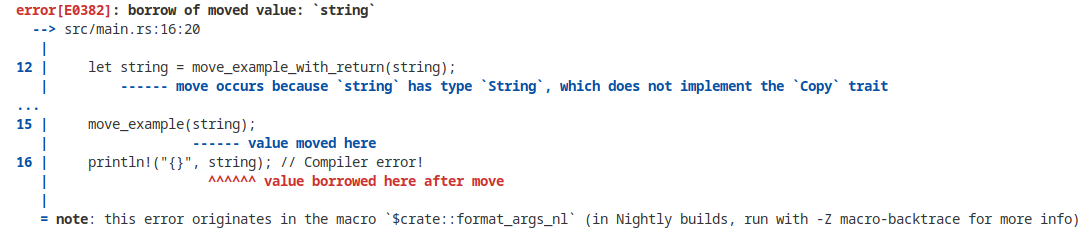
\includegraphics[scale=0.55]{kuvat/move_error_light.png}}
  \caption{Resurssin käyttöyritys siirron jälkeen johtaa käännösvirheeseen.}
  \label{rust_move_image}
\end{figure}

Omistajuuden siirtymisen voi välttää käyttämällä viittauksia (engl. reference) resursseihin. Viittaukset ovat oletuksena muuttumattomia, mutta Rustissa on myös mahdollista tehdä viittauksia, jonka kautta arvoa voi muokata~\cite[p.~147]{10.1145/3418295}. Rustin kääntäjän lainausten tarkistaja (engl. borrow checker) tarkistaa, että resurssiin on kulloinkin olemassa vain joko muuttumattomia viittauksia tai tasan yksi muokattavissa oleva viittaus~\cite[chapter~4.2]{rustbook}. Samaan resurssiin ei voi olla samanaikaisesti olemassa muuttumattomia ja muokattavissa olevia viittauksia. Viittausten rajoittaminen tällä tavalla estää kilpailutilanteiden synnyn, vaikka resurssia muokattaisiinkin viittauksen kautta. Ohjelmoija voi olla varma, että muuttumattoman viittauksen osoittama arvo ei voi muuttua, niin kauan kun viittaus on olemassa~\cite[chapter~4.2]{rustbook}. Viittauksilla resurssin voi antaa argumenttina funktiolle ja jatkaa sen käyttöä myöhemmin, ilman että funktion tulee palauttaa resurssin omistajuutta.

Rustissa jokaisella viittauksella on elinaika (engl. lifetime), jonka tarkoitus on varmistaa, että viittaukset ovat olemassa niin kauan kuin niitä tarvitaan. Kääntäjä osaa usein päätellä elinajan automaattisesti, mutta joskus ohjelmoijan täytyy itse kertoa kääntäjällä viittauksen elinaika. Elinajan merkintä kertoo kääntäjälle, että kaikki saman elinajan omaavat viittaukset ovat voimassa vähintään elinajan verran. Elinajasta Rustissa huolehtii lainausten tarkistaja, joka vertaa elinaikoja keskenään ja tarkistaa viittausten voimassaolon. Elinajan ja lainaustarkistajan ansiosta roikkuvaa osoitinta (engl. dangling pointer) eli osoitinta, jonka osoittama muistialue on siirtynyt toisen osoittimen käyttöön, ei voi syntyä. Rustissa on myös erityinen elinaika \textit{'static}, joka tarkoittaa viittauksen olevan voimassa koko ohjelman elinajan.~\cite[chapter~10.3]{rustbook}

Ohjelmalistaus \ref{lifetime_rust} ja kuva \ref{lifetime_error_rust} esittelevät elinajan ilmoittamisen eksplisiittisesti ja kääntäjän antaman virheen, mikäli se ei osaa päätellä elinaikaa. Elinajan ilmoittaminen on pakollista listauksessa, koska kääntäjä ei tiedä käännösvaiheessa, onko funktiosta palautuva viittaus \textit{str1} vai \textit{str2}, jolloin kääntäjälle tulee ilmoittaa, että molemmat ovat olemassa yhtä kauan kuin palautettava viittaus.

\begin{minipage}{\linewidth}
\lstinputlisting[language=rust, caption=Elinajan ilmoittaminen Rustissa., label={lifetime_rust}]{koodiesimerkit/lifetimes.rs}
\end{minipage}

\begin{figure}[h]
  \frame{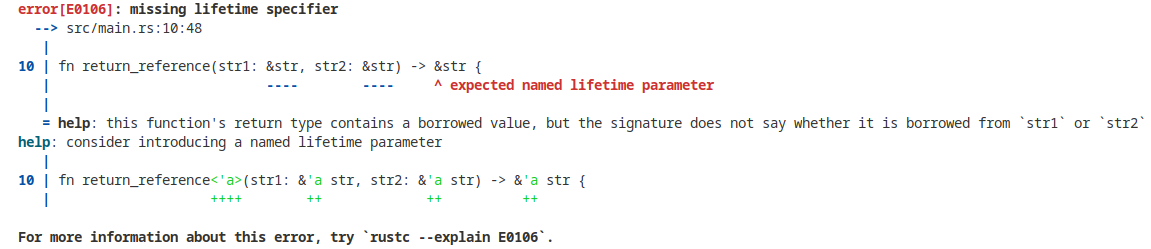
\includegraphics[scale=0.55]{kuvat/lifetime_error_light.png}}
  \caption{Kääntäjä ei osaa päätellä elinaikaa, joten sen poisjättäminen johtaisi virheeseen.}
  \label{lifetime_error_rust}
\end{figure}

\section{Säikeet}
Rust mahdollistaa säikeiden käytön tarjoamalla rajapinnan, jonka kautta säikeiden käyttäminen on turvallista. Rustin omistajuusjärjestelmä takaa, että resurssin omistajuus on yhdellä säikeellä, jolloin moni säie ei voi muokata samaa resurssia. Näin voidaan välttää kilpailutilanteet montaakin säiettä käytettäessä~\cite[chapter~16]{rustbook}. 

Rust myös mahdollistaa tilan jakamisen ja omistajuuden siirtämisen säikeiden välillä käyttämällä viestintäkanavia, joiden avulla resurssi ja sen omistajuus voidaan siirtää säikeeltä toiselle~\cite[chapter~16.2]{rustbook}. Kanavien lisäksi säikeet voivat jakaa tilan hyödyntämällä lukkiutuvia tyyppejä kuten Mutex- ja Arc-tyyppejä. Rustin kääntäjä varmistaa, että jaettuja resursseja käytetään säieturvallisesti älykkäiden osoittimien kautta~\cite[chapter~16.3]{rustbook}. Ohjelmalistaus \ref{rust_thread} esittelee jaetun resurssin käyttöä säikeissä Rustissa.


\begin{minipage}{\linewidth}
\lstinputlisting[language=rust, caption=Tilan jakaminen säikeissä Arc- ja Mutex-tyyppien avulla., label={rust_thread}]{koodiesimerkit/threads.rs}
\end{minipage}

\section{Cargo-pakettihallinta}
Rust sisältää kappaleessa \ref{kirjastot} mainitun Cargo-nimisen pakettihallintaohjelman, joka mahdollistaa kirjastojen sisällyttämisen ohjelmaan helposti. Cargon avulla projektin riippuvuuksia voidaan päivittää tai niiden versiota alentaa, jolloin kirjastojen aiheuttamia ongelmia on helppo paikata esimerkiksi tilanteessa, jossa kirjaston ylläpitäjä paikkaa löydetyn haavoittuvuuden ja päivitys halutaan mahdollisimman nopeasti sisällyttää kirjastoa käyttävään ohjelmaan. Cargolla voi asentaa riippuvuuksia crates io-rekisteristä, versionhallintapalveluista tai paikallisesti. Kirjastot ja niiden versiot määritetään Cargo.toml-tiedostoon käyttäen Semver-syntaksia, jolla voidaan määrittää sallitut versionumerot kirjastoille. Cargo luo Cargo.lock tiedoston, jossa on kyseisen ohjelman käyttämät kirjastot ja niiden käytössä olevat versiot. Kirjastot voi päivittää \textit{cargo update}-komennolla, jolloin kaikki kirjastot päivittyvät korkeimpaan Cargo.toml tiedostossa sallittuun versioon.

\section{Rustin heikkoudet}
Rustin turvajärjestelmät eivät pysty ratkaisemaan kaikkia C-kielien haasteita eivätkä ne myöskään estä ohjelmoijaa tekemästä virheitä. Esimerkiksi muistivuoto on mahdollista Rustissa luomalla kiertävä viittaus (engl. cyclic reference), jossa toisiinsa viittaavat indeksit aiheuttavat sen, että indeksille varattua muistia ei koskaan vapauteta~\cite[chapter~15.6]{rustbook}. Rustissa kiertävän viittauksen luoma ongelma voidaan ratkaista käyttämällä heikkoa viittausta Weak<T>-osoittimen avulla. Heikko viittaus ei estä resurssin pudottamista, minkä johdosta toisiinsa viittaavat indeksit pudotetaan samaan aikaan niiden osoittimien kanssa. Kuva \ref{cyclic_reference} havainnollistaa kiertävän viittauksen luomaa muistivuotoa.

\begin{figure}[H]
  \frame{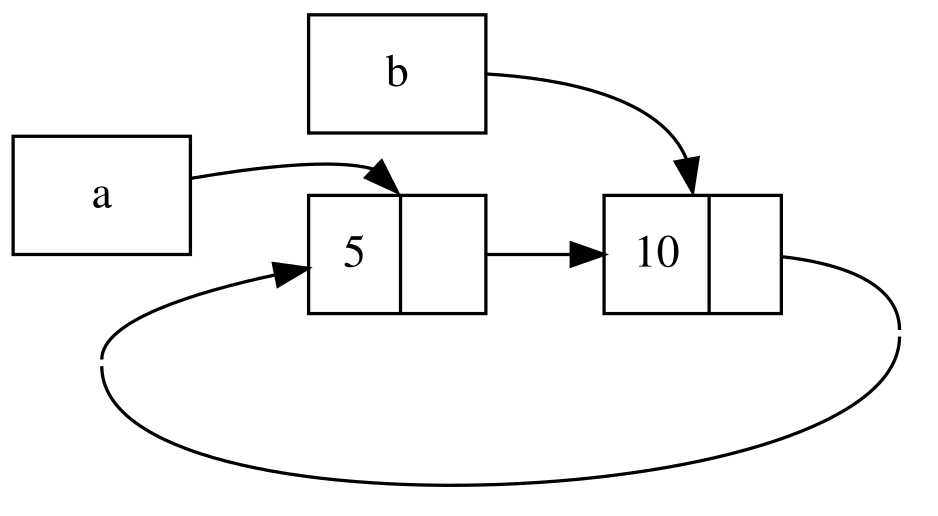
\includegraphics[scale=0.55]{kuvat/cyclic.png}}
  \caption{Kiertävässä viittauksessa muistia ei vapauteta, vaikka a ja b pudotetaan, sillä niiden osoittamat indeksit viittaavat toisiinsa~\cite[chapter~15.6]{rustbook}.}
  \label{cyclic_reference}
\end{figure}

Muistivuodon lisäksi säikeiden lukkiutumistilanne on mahdollinen ongelma Rustissa, sillä mikään Rustin turvajärjestelmistä ei estä tilannetta, jossa säikeet odottavat toistensa käyttämän resurssin vapautumista. Rustin turvajärjestelmät voivat johtaa lisäksi pitempään kehitysaikaan, minkä johdosta se ei välttämättä sovellu kovin hyvin konseptin todennukseen (engl. proof of concept) tai muihin lyhyisiin projekteihin, joissa koodin oikeellisuus ja kaikkien virhetilanteiden huomioiminen ei ole oleellista. 

Rustin opettelu voi myös viedä paljon aikaa, jolloin sen käyttöönotto ei välttämättä suju kovin helposti. Tästä johtuen Rustin käyttöönoton perustelu voi olla haastavaa esimerkiksi yritysmaailmassa. Lisäksi Rust-kielen osaajia voi olla vaikea löytää, jolloin voi syntyä tilanne, jossa Rustia ei nähdä järkevänä opetella, koska sille ei löydy työpaikkoja, eikä Rustia oteta käyttöön, koska sillä ei ole tarpeeksi osaajia. Rustin viralliset sivut tarjoavat kuitenkin paljon opetusmateriaalia eri tasoisille kielen osaajille, mikä helpottaa opettelua.

Rustin ekosysteemi on vielä nuori, joten on mahdollista, että jollekin kehittäjän haluamalle toiminnallisuudelle tai integraatiolle ei ole vielä valmista kirjastoa tai kirjasto ei ole vielä vakaa, jolloin kehittäjän täytyy joko kirjoittaa oma kirjasto tai turvautua toisella kielellä tehtyyn integraatioon, jolloin Rustin tarjoamat turvaominaisuudet menetetään kyseisen toiminnallisuuden osalta. Rust kuitenkin mahdollistaa tämän FFI:n eli Foreign Function Interfacen kautta, jonka avulla voidaan kutsua toisella kielellä kirjoitettuja funktioita.

Tiettyjen tietorakenteiden toteuttaminen Rustissa voi osoittautua turvaominaisuuksien takia hankalaksi, mikä puolestaan voi johtaa unsafe-tilan suosimiseen, jossa osa kääntäjän turvallisuusominaisuuksista kytketään pois päältä~\cite[chapter~19.1]{rustbook}. Tutkimus kehittäjien unsafe-tilan käyttöön havaitsi, että suurin osa crates.io:sta löytyvistä kirjastoista käyttää unsafe-tilaa jossakin muodossa, mutta suurimassa osassa se on abstraktoitu turvallisen rajapinnan taakse, jolloin kirjaston käyttäjän ei tarvitse käyttää unsafe-tilaa omassa koodissaan~\cite[p.~252]{unsafe}. Unsafe-tilan käyttö saattaa olla tietyissä matalan tason operaatioissa pakollista, mutta suurimmassa osassa ohjelmia sen käyttö on tarpeetonta. Unsafe tila ei myöskään poista lainauksen tarkistajaa ja omistajuutta käytöstä vaan se vaikuttaa vain muistiturvallisuustakuisiin~\cite[chapter~19.1]{rustbook}.